% !TEX encoding = UTF-8 Unicode
\documentclass[convert={density=300,size=1000x700,outext=.png}]{standalone}
\usepackage{tikz}
% \usepackage[active,tightpage,psfixbb]{preview}
\usepackage{tipa,dingbat}
% \PreviewEnvironment{pgfpicture}
% \setlength\PreviewBorder{2pt}
\usetikzlibrary{positioning, shapes}



\begin{document}
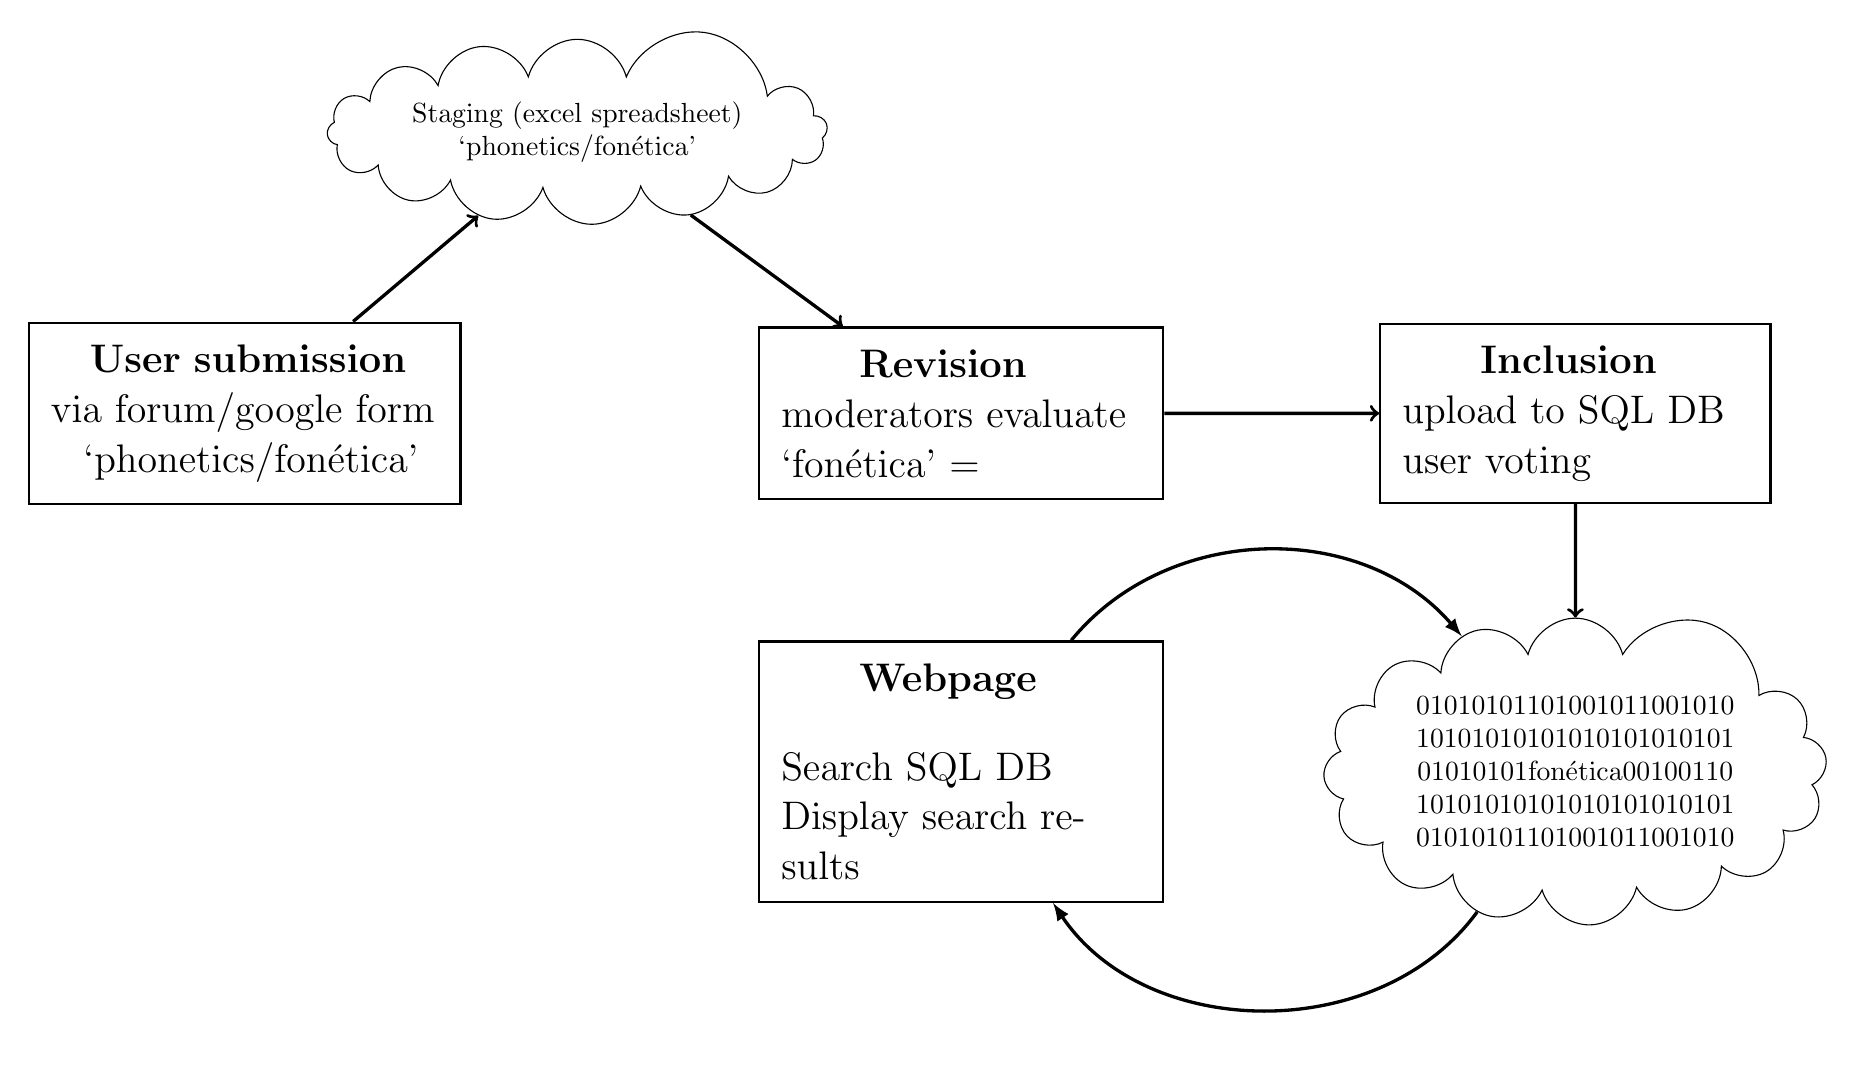
\begin{tikzpicture}[scale=.65]

% \draw[help lines] (0,0) grid (38,31);

\tikzstyle{gbox1}=[draw=black, thick,shape=rectangle,inner sep=8pt,
text width=14em, text height=1em, font=\Large];
\tikzstyle{gbox2}=[draw=black, thick,shape=rectangle,inner sep=8pt,
text width=13em, text height=1em, font=\Large];
\tikzstyle{gbox3}=[draw=black, thick,shape=rectangle,inner sep=8pt,
text width=12.5em, text height=1em, font=\Large];
\tikzstyle{gbox4}=[draw=black, thick,shape=rectangle,inner sep=8pt,
text width=13em, text height=1em, font=\Large];


\node[gbox1] (a1) at (1,15) {\hspace{1em}\textbf{User submission} \\ via forum/google form \\ \hspace{.5em} `phonetics/fon\'etica'};
\node[cloud, cloud puffs=15.7, cloud ignores aspect, minimum width=5cm, minimum height=2cm, align=center, draw] (a2) at (7.5,20.5) {Staging (excel spreadsheet) \\ `phonetics/fon\'etica'};
\node[gbox2] (a3) at (15,15) {\hspace{2em}\textbf{Revision} \\ moderators evaluate \\ `fon\'etica' = \leftthumbsup};
\node[gbox3] (a4) at (27,15) {\hspace{2em}\textbf{Inclusion} \\ upload to SQL DB \\ user voting \leftthumbsup \leftthumbsdown};
\node[cloud, cloud puffs=15.7, cloud ignores aspect, minimum width=5cm, minimum height=2cm, align=center, draw] (a6) at (27,8) {01010101101001011001010\\10101010101010101010101\\01010101fon\'etica00100110\\10101010101010101010101\\01010101101001011001010};
\node[gbox4] (a5) at (15,8) {\hspace{2em}\textbf{Webpage} \\ \vspace{1em} Search SQL DB\\ Display search results};

% lines
\draw [->, very thick] (a1) -- (a2);
\draw [->, very thick] (a2) -- (a3);
\draw [->, very thick] (a3) -- (a4);
\draw [->, very thick] (a4) -- (a6);

\draw [-latex, very thick] (a5) to[bend left=50] (a6) ;
\draw [-latex, very thick] (a6) to[bend left=55] (a5) ;








\end{tikzpicture}
\end{document}